\documentclass[8pt]{article}
\usepackage{fullpage}
\usepackage{amsmath}
\usepackage{amssymb}
\usepackage[usenames]{color}
\usepackage{fontspec}
\usepackage{fontawesome}
\usepackage{hyperref}
\usepackage[normalem]{ulem}
\usepackage{tikz}
\usetikzlibrary{calc}
\usepackage{eso-pic}

% --- Document metadata: gives ATS / AI PDF parsers reliable Title, Author,
% --- language, and keyword hints from the PDF's /Info + XMP streams.
\hypersetup{
  pdftitle={Tyler Alamo Port -- Software Engineer Resume},
  pdfauthor={Tyler Alamo Port},
  pdfsubject={Software Engineer Resume},
  pdfcreator={Tyler Alamo Port},
  pdflang={en-US},
  pdfkeywords={Software Engineer, Rust, Python, C, C++, CUDA, SYCL, OpenCL, HIP,
    GPU Programming, High-Performance Computing, HPC, FPGA, Systems Engineering,
    Image Processing, Imaging, Computer Vision, React, Docker,
    DevOps, Infrastructure, Tauri, Leptos, WebAssembly, Nix, Terraform,
    GSSAPI, Kerberos, SQL, PostgreSQL, Caltech, Elysian Studio, ElyMalloc, ElyLD,
    Allocator, Linker, ELF, mimalloc, wgpu},
  hidelinks
}

% Keep glyph-to-Unicode mapping intact so copied/extracted text is clean,
% and never break words across lines (hyphenation confuses naive parsers).
\hyphenpenalty=10000
\exhyphenpenalty=10000

% --- Subtle technical background -------------------------------------------
% Drawn as vector graphics in the page background only. It carries NO text,
% so the PDF text layer (what AI/ATS systems extract) is completely unaffected,
% and the very low ink density keeps all foreground text fully legible.
\newcommand{\circuitmotif}{%
  \begin{scope}[line width=0.45pt, draw=blue!13, fill=blue!13,
                line cap=round, line join=round]
    \draw (0,0) -- (1.6,0) -- (1.6,-0.9) -- (2.8,-0.9);
    \draw (0,-0.5) -- (1.1,-0.5) -- (1.1,-1.7) -- (2.4,-1.7);
    \draw (0.6,0) -- (0.6,-2.2) -- (2.0,-2.2);
    \foreach \p in {(0,0),(1.6,0),(1.6,-0.9),(2.8,-0.9),%
                    (1.1,-1.7),(2.4,-1.7),(0.6,-2.2),(2.0,-2.2)}{%
      \fill \p circle (1.3pt);
    }
  \end{scope}%
}
\AddToShipoutPictureBG*{%
  \begin{tikzpicture}[overlay, remember picture]
    \begin{scope}
      \clip (current page.south west) rectangle (current page.north east);
      \draw[line width=0.2pt, black!5, step=0.55cm]
        (current page.south west) grid (current page.north east);
      \begin{scope}[shift={($(current page.north west)+(1.0cm,-1.3cm)$)}]
        \circuitmotif
      \end{scope}
      \begin{scope}[shift={($(current page.south east)+(-1.0cm,1.3cm)$)}, rotate=180]
        \circuitmotif
      \end{scope}
    \end{scope}
  \end{tikzpicture}%
}

\leftmargin=0.1in
\oddsidemargin=0.10in
\textwidth=6.0in
\topmargin=-0.35in
\textheight=9.55in

\raggedright

%\pagenumbering{arabic}
\pagenumbering{gobble}

\def\bull{\vrule height 0.8ex width .7ex depth -.1ex }
% DEFINITIONS FOR RESUME

\newenvironment{changemargin}[2]{%
  \begin{list}{}{%
    \setlength{\topsep}{0pt}%
    \setlength{\leftmargin}{#1}%
    \setlength{\rightmargin}{#2}%
    \setlength{\listparindent}{\parindent}%
    \setlength{\itemindent}{\parindent}%
    \setlength{\parsep}{0pt}%
    \setlength{\itemsep}{-2pt}%
  }%
  \item[]}{\end{list}
}

\newcommand{\lineover}{
	\begin{changemargin}{-0.05in}{-0.05in}
		\vspace*{-10pt}
		\hrulefill \\
		\vspace*{-4pt}
	\end{changemargin}
}

\newcommand{\header}[1]{
	\begin{changemargin}{-0.5in}{-0.5in}
		\scshape{#1}\\
  	\lineover
	\end{changemargin}
}

\newcommand{\contact}[4]{
	\begin{changemargin}{-0.5in}{-0.5in}
		\begin{center}
			{\Large \scshape {#1}}\\ \smallskip
			{#2}\\ \smallskip 
			{#3}\\ \smallskip
			{#4}\smallskip
		\end{center}
	\end{changemargin}
}

\newenvironment{body} {
	\vspace*{-10pt}
	\begin{changemargin}{-0.25in}{-0.5in}
  }	
	{\end{changemargin}
}	

\newcommand{\school}[4]{
	\textbf{#1} \hfill \emph{#2\\}
	#3\\ 
	#4\\
}

% END RESUME DEFINITIONS

\begin{document}
%%%%%%%%%%%%%%%%%%%%%%%%%%%%%%%%%%%%%%%%%%%%%%%%%%%%%%%%%%%%%%%%%%%%%%%%%%%%%%%%
% Contact Info
\begin{center}
	\vspace*{-48pt}
	{\Large \scshape Tyler Alamo Port}
\end{center}
\vspace*{-4pt}
\hspace{7.25mm} \faGithub \hspace{0.25mm} \textbf{\href{https://github.com/tyler274}{github.com/tyler274}} \hspace{7.25mm} \faLinkedinSquare \hspace{0.25mm} \textbf{\href{https://linkedin.com/in/tyler-port-9a795455/}{linkedin.com/in/tyler-port-9a795455}} \\
\vspace*{1pt}  \hspace{12.25mm} \faEnvelope \hspace{0.1mm} \textbf{\href{mailto:tp@dabney.moe}{tp@dabney.moe}} \hspace{8.25mm} \faGlobe \hspace{0.1mm} \textbf{\href{https://dabney.moe}{dabney.moe}} \hspace{8.25mm} \faMobile : \textbf{\href{tel:+15167767470}{+1 (516) 776-7470}}\\
\vspace*{-11pt}
\smallskip

%%%%%%%%%%%%%%%%%%%%%%%%%%%%%%%%%%%%%%%%%%%%%%%%%%%%%%%%%%%%%%%%%%%%%%%%%%%%%%%%
% Education
\header{Education}
%\smallskip
\begin{body}
	\vspace{10pt}
	\textbf{California Inst. of Technology [Caltech]}{}, \emph{B.S. in
	\textbf{Computer Science}:} \hfill \emph{Jun. 2022}{} \\
	\vspace{-5pt}
	\begin{itemize} \itemsep -2pt
		\item Focused on low-level GPU programming for parallel algorithm acceleration; taught GPU Programming and Rust.
	\end{itemize}
\end{body}

\smallskip
\vspace*{-11pt}

%%%%%%%%%%%%%%%%%%%%%%%%%%%%%%%%%%%%%%%%%%%%%%%%%%%%%%%%%%%%%%%%%%%%%%%%%%%%%%%%
% Experience
\header{Work and Experience}
\begin{body}
	\vspace{10pt} % Reduced space

	\textbf{Tivara, New York City}, \emph{Founding Software Engineer} \hfill \emph{May 2025 - August 2025}\\
	\vspace*{-6pt}
	\begin{itemize} \itemsep -2pt
		\item Oversaw end-to-end development, and launched the product pilots, of AI voice agents for patient intake and
		scheduling for two clinical networks situated across the United States.
		\item Full-stack development of the clinician-facing product in TypeScript, React, and Node.js: intake and
		scheduling UI, APIs, and pilot infrastructure and operations.
		% \item Engaged in full-stack development, systems integration, and performance optimization for various freelance contracts. % Optional 3rd point if space allows
	\end{itemize}
	\vspace*{-6pt}

	\textbf{Freelance Engineer and Independent Game Developer} \hfill \emph{October 2024 - Present}\\
	\vspace*{-6pt}
	\begin{itemize} \itemsep -2pt
		\item Building \href{https://github.com/tyler274/elysian-studio}{Elysian Studio}, \href{https://github.com/tyler274/ElyMalloc}{ElyMalloc}, and \href{https://github.com/tyler274/ElyLD}{ElyLD}: a safe-Rust slicer, allocator, and incremental ELF linker (see Projects).
		\item Leading a from-scratch Rust rewrite of \texttt{gssproxy}, the GSSAPI/Kerberos proxy daemon and its mechglue interposer: a memory-safe, drop-in replacement across a multi-crate workspace, with FFI to MIT krb5/GSSAPI and Kani formal verification of the security-critical XDR/gssx wire codec.
		\item Built \href{https://dabney.moe}{dabney.moe} as a Leptos (SSR + WASM) and Tauri v2 multiplatform app sharing one Rust UI crate. Leptos is a reactive component framework similar to Vue.js: components, fine-grained reactivity, and server rendering. Nix-driven multi-cloud (GCP/AWS/Azure) Terraform CI/CD publishes hardened, statically linked Docker images.
	\end{itemize}
	\vspace*{-6pt}

	\textbf{Carl Zeiss AG., Germany}, \emph{System Software Engineer} \hfill \emph{March 2023 - March 2024}\\
	\vspace*{-6pt} % Reduced space
	\begin{itemize} \itemsep -2pt % Ensure negative itemsep
		\item Led systems engineering for imaging and computer-vision workloads on GPUs and FPGAs, using CUDA C++, SYCL, and Python to accelerate scientific image processing and machine-learning inference.
		\item Managed master's students and interns on GPU/FPGA programming and real-time imaging-pipeline optimization.
		\item Developed, deployed, and tested FPGA implementations of PyTorch models for real-time image-signal-processing and computer-vision pipelines.
	\end{itemize}
	\vspace*{-6pt}

	\textbf{Caltech}, \emph{Lecturer and Teaching Assistant in Computer Science} \hfill \emph{April 2018 - June 2022}\\
	\vspace*{-6pt}
	\begin{itemize} \itemsep -2pt
		\item Taught and developed material for CS179 (GPU Programming, Nvidia CUDA), the CS11 Rust workshop (reimplementing CS24 Operating Systems assignments from C to Rust), and CS121 (relational database theory and SQL).
	\end{itemize}
	\vspace*{-6pt}

	\textbf{Tinder Inc.}, \emph{Software Engineering Intern} \hfill \emph{June 2018 - August 2018}\\
	\vspace*{-5pt}
	\begin{itemize} \itemsep -2pt
		\item Developed Prometheus/Grafana extension (Python, Puppet) to trace microservice dependencies and identify root causes of service degradation.
	\end{itemize}
	\vspace*{-6pt}

	\textbf{NASA Jet Propulsion Lab}, \emph{Software Engineering Intern} \hfill \emph{January 2018 - June 2018}\\
	\vspace*{-5pt}
	\begin{itemize} \itemsep -2pt
		\item Accelerated Europa Lander orbital calculations via MATLAB-to-CUDA C++ reimplementation for large-scale parallel simulation/visualization.
	\end{itemize}
	\vspace*{-6pt}

	\textbf{Caltech IMSS}, \emph{IMSS Representative and UGCS Systems Administrator} \hfill \emph{January 2016 - June 2022}\\
	\vspace*{-6pt}
	\begin{itemize} \itemsep -2pt
		\item Administered 150TB storage array and compute resources, ensuring high availability/performance for thousands of users (Linux environment).
	\end{itemize}
	\vspace*{-6pt}

	\textbf{KarmaFleet}, \emph{Director of Technology} \hfill \emph{January 2015 - September 2016}\\
	\vspace*{-6pt}
	\begin{itemize} \itemsep -2pt
		\item Architected/developed Python/Flask/SQLAlchemy/PostgreSQL web app for 4500+ users; implemented DevOps (Docker, CI, monitoring) and managed critical infrastructure (VoIP, forums, chat).
	\end{itemize}
	\vspace*{-6pt}

\end{body}

\vspace*{-6pt}

%%%%%%%%%%%%%%%%%%%%%%%%%%%%%%%%%%%%%%%%%%%%%%%%%%%%%%%%%%%%%%%%%%%%%%%%%%%%%%%%
% Projects
\header{Projects}
\begin{body}
	\vspace{8pt}
	\begin{itemize} \itemsep -2pt
		\item \textbf{\href{https://github.com/tyler274/elysian-studio}{Elysian Studio}}: AGPL safe-Rust rewrite of Bambu Studio; integer-deterministic CPU slicing, wgpu Vulkan compute contours, iced UI, and open LAN printer I/O.
		\item \textbf{\href{https://github.com/tyler274/ElyMalloc}{ElyMalloc}}: Pure-Rust drop-in for Microsoft mimalloc v3.5.2 (\texttt{libmimalloc.so.3}, \texttt{mi\_*}) with always-on \texttt{MI\_SECURE} mitigations, WASM \texttt{GlobalAlloc}, Kani proofs, and a NixOS malloc provider.
		\item \textbf{\href{https://github.com/tyler274/ElyLD}{ElyLD}}: GNU-ld-compatible incremental ELF linker (Wild fork); \texttt{--incremental} in-place patching, Linux kernel \texttt{vmlinux}, glibc DSOs, and NixOS stdenv linker.
	\end{itemize}
\end{body}

\vspace*{-8pt}

%%%%%%%%%%%%%%%%%%%%%%%%%%%%%%%%%%%%%%%%%%%%%%%%%%%%%%%%%%%%%%%%%%%%%%%%%%%%%%%%
% Skills
\header{Skills}
\begin{body}
	\vspace{8pt}
	\begin{itemize} \itemsep -2pt
		\item \uline{Languages:} \textbf{Rust}, \textbf{Python}, \textbf{C/C++},
		\textbf{CUDA/SYCL/OpenCL/HIP (GPU Programming)}, SQL, C\#, Java/Kotlin, TypeScript/JavaScript, React,
		Haskell, OCaml, VHDL, Mathematica.
		\item \uline{Platforms/Technology:} Linux (Gentoo, Arch, RHEL/Fedora, Debian/Ubuntu), HPC Environments, FPGAs (Intel, AMD), Docker, Git, Windows, MacOS, BSD.
		\item \uline{Specialties:} \textbf{GPU Computing \& Parallelization}, \textbf{Image Processing, Imaging \& Computer Vision}, \textbf{Systems Engineering \& Administration}, \textbf{DevOps \& Infrastructure Management (Docker)}, High-Performance Computing (HPC), Memory Allocators, ELF Linkers, AI/Machine Learning (PyTorch), React, Low-Level Programming, Relational Database Design (SQL, PostgreSQL), Functional Programming, Computer Graphics.
	\end{itemize}
\end{body}

\end{document}
